
\documentclass[11pt,a4paper]{article}
\usepackage[utf8]{inputenc}
%\usepackage[icelandic]{babel}
%\usepackage[T1]{fontenc}
\usepackage{amsmath}
\usepackage{amsfonts}
\usepackage{amssymb}
%\usepackage{graphicx}
%\author{Arnar Ingi Halldórsson}
%\title{Linear Motion}


%\documentclass{article}
\usepackage{graphicx}
\graphicspath{ {myndir/} }
\usepackage[T1]{fontenc} 
\usepackage[english]{babel}

\usepackage[utf8]{inputenc} 
\usepackage{graphics}
%\usepackage[pdftex]{graphicx}

\usepackage{caption}
\usepackage{subcaption}

\usepackage{titling}

\setlength{\droptitle}{-10em}
   
\title{Assignment 1 \\ T-509-RAFT \\ Electronics} % Title

\author{Arnar Ingi Halldórsson \\ Hjörleifur G Bergsteinsson \\ Snorri Stefánsson} % Author name
\begin{document}

\maketitle % Insert the title, author and date

\begin{tabular}{lr}
Due date: 22.02.2015 \\
Teachers:\qquad Slawomir Koziel\\ % Instructor/supervisor
\qquad \qquad \qquad Adrian Bekasiewicz
\end{tabular}

\setlength\parindent{0pt} % Removes all indentation from paragraphs

\renewcommand{\labelenumi}{\alph{enumi}.} % Make numbering in the enumerate environment by letter rather than number (e.g. section 6)

\section*{Introduction}


\section*{Task 1: Perfomance Parameters of Op Amp}

\begin{enumerate}
  \item[1.]
		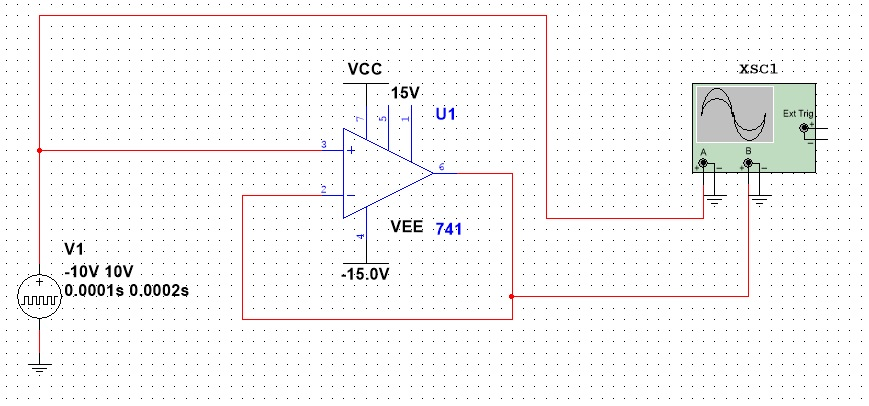
\includegraphics[width=10cm]{Task1-1Circuit}\\
		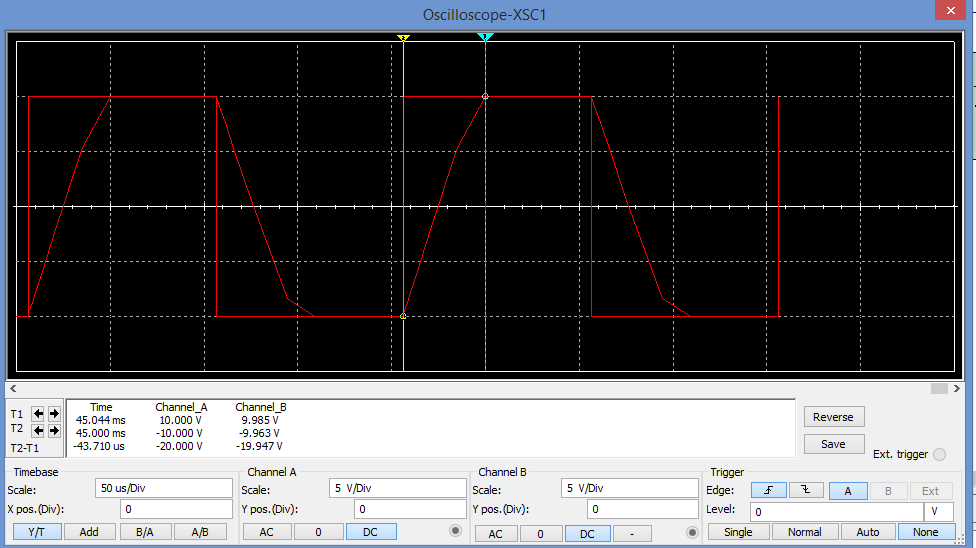
\includegraphics[width=10cm]{Task1-1-Oscilloscope}
  
  \item[2.]
  		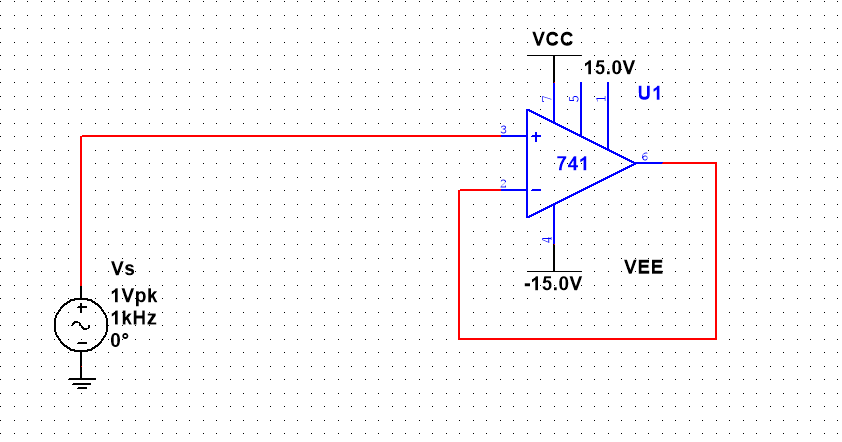
\includegraphics[width=10cm]{Task1-2-Circuit}\\
		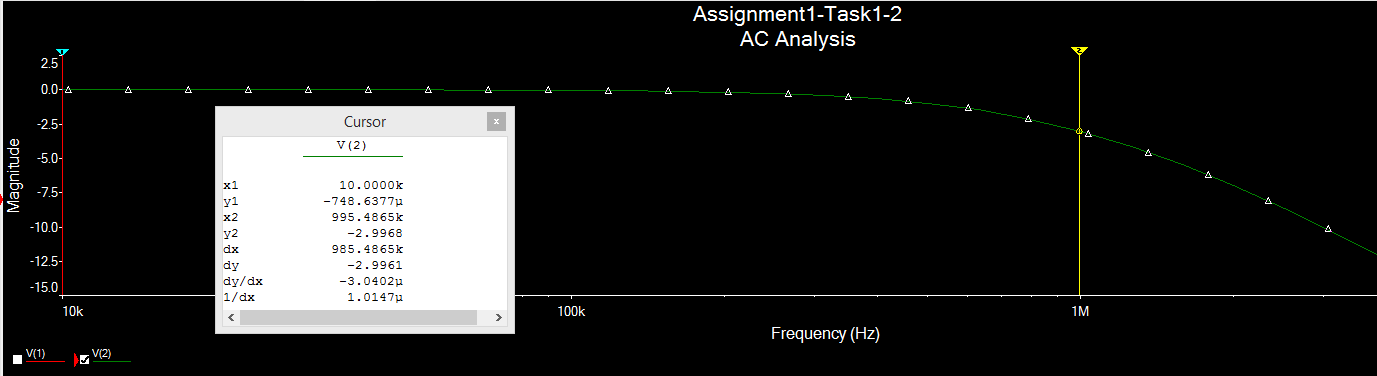
\includegraphics[width=10cm]{Task1-2-ACAnalysis}
  \item[3.]
    	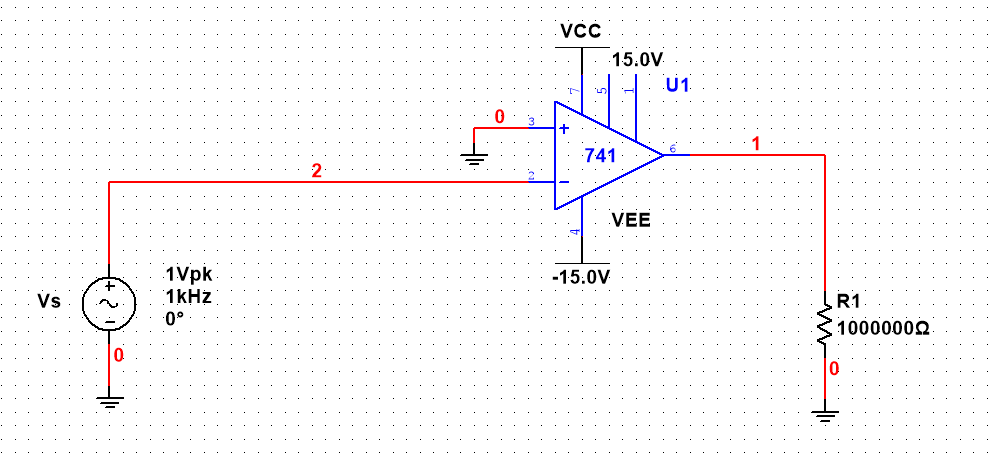
\includegraphics[width=10cm]{Task1-3-Circuit}\\
		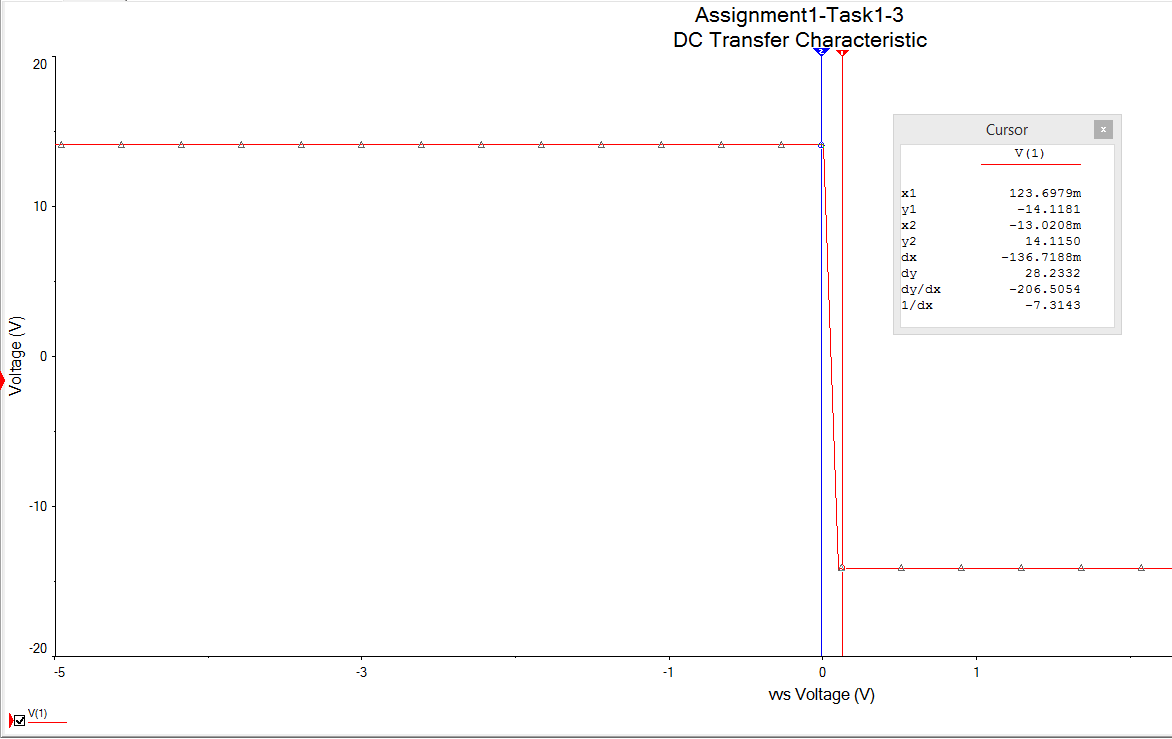
\includegraphics[width=10cm]{Task1-3-DCAnalysis}
  \item[4.]
  
	\begin{tabular}{l*{3}{c}r}
	$\mu$ A741 op-Amp              & DataSheet & Simulation  \\
	\hline
	Slew Rate [$SR$]   & 6 & 4 \\
	Gain-Bandwidth [$GBW$]              & 6 & 3 \\
	DC Differential Gain [$A_{d}$]             & 6 & 2 \\
	Input Offset Voltage [$V_{os}$]           & 6 & 2 \\
	\end{tabular}

\end{enumerate}

\section*{Task 2: Frequency Response of Inverting Amplifier}

\begin{enumerate}
  \item[1.]
  
  \item[2.]
  
\end{enumerate}

\section*{Task 3: Op Amplifies Design}

\begin{enumerate}
  \item[1.]
  
  \item[2.]
  
  \item[3.]
  
\end{enumerate}

\section*{Task 4: Half - Wave Rectifier}

\begin{enumerate}
  \item[1.]
  
  \item[2.]
  
  \item[3.]
  
\end{enumerate}


\end{document}
\\
